\documentclass[letterpaper]{article}

\usepackage{aaai}
\usepackage{times}
\usepackage{helvet}
\usepackage{courier}
%%%%%%%%%%
% PDFMARK for TeX and GhostScript
% Uncomment and complete the following for
% metadata if your paper is typeset using TeX and
% GhostScript (e.g if you use .ps or .eps files in your paper):
\special{! /pdfmark where
{pop} {userdict /pdfmark /cleartomark load put} ifelse
[ /Author (Christopher Weber, Daniel Bryce)
 /Title (Planning and Acting in Incomplete Domains)
 /Subject (International Conference on Automated Planning and Scheduling)
 /Keywords (Planning, Execution, Learning, Uncertainty)
 /DOCINFO pdfmark
} 
%%%%%%%%%%
\setcounter{secnumdepth}{1}

\usepackage{graphicx}
\usepackage[linesnumbered,ruled,vlined]{algorithm2e}
\usepackage{multirow}
\usepackage{amsmath, amsthm, amssymb}
\newenvironment{packed_enum}{
\begin{enumerate}
  \setlength{\itemsep}{1pt}
  \setlength{\parskip}{0pt}
  \setlength{\parsep}{0pt}
}{\end{enumerate}}
\newenvironment{packed_itemize}{
\begin{itemize}
  \setlength{\itemsep}{1pt}
  \setlength{\parskip}{0pt}
  \setlength{\parsep}{0pt}
}{\end{itemize}}


\def\und#1{\noindent{\bf #1}:}
\def\default{{\tt DeFault}} 
\def\goalie{{\tt Goalie}}
\def\citep#1{\cite{#1}} 
\def\citet#1{\citeauthor{#1} (\citeyear{#1})}




\begin{document}
\title{Planning and Acting in Incomplete Domains}

\author{
Christopher Weber \and Daniel Bryce\\
christopherweber@hotmail.com, daniel.bryce@usu.edu\\
Department of Computer Science\\
Utah State University
}

\maketitle

\begin{abstract}
Engineering complete planning domain descriptions is often very costly because
of human error or lack of domain knowledge. Learning complete domain
descriptions is also very challenging because many features are irrelevant to
achieving the goals and data may be scarce.  We present a planner and agent
that respectively plan and act in incomplete domains by i) synthesizing plans
to avoid execution failure due to ignorance of the domain model, and ii) passively learning about the
domain model during execution to improve later re-planning attempts.

Our planner \default{} is the first to reason about a domain's incompleteness to
avoid potential plan failure.  \default{} computes failure explanations for each
action and state in the plan and counts the number of interpretations of the
incomplete domain where failure will occur. We show that \default{} performs
best by counting  prime implicants (failure diagnoses) rather than propositional
models. Our agent \goalie{} learns about the preconditions and effects of
incompletely-specified actions while monitoring its state and, in conjunction
with \default{} plan failure explanations, can diagnose past and future action
failures.   We show that by reasoning about incompleteness (as
opposed to ignoring it) \goalie{} fails and re-plans less and executes fewer
actions.

\end{abstract}


\section{Introduction}
The knowledge engineering required to create complete and correct domain
descriptions for planning problems is often very costly and difficult
\citep{modellite,arms}.  Machine learning techniques have been applied with some
success \citep{arms}, but still suffer from impoverished data and limitations of
the algorithms \citep{modellite}.   In particular, we are motivated by
applications in instructable computing \citep{mable} where a domain expert
teaches an intelligent system about a domain, but can often leave out whole
procedures (plans) and aspects of action descriptions.   In such cases, the
alternative to making domains complete is to plan around the incompleteness. 
That is, given knowledge of the possible action descriptions, we seek out plans
that will succeed despite any (or most of the) incompleteness in the domain
formulation.

While prior work \citep{Garland02} (henceforth abbreviated, GL) has categorized
risks to a plan and described plan quality metrics in terms of the risks
(essentially single-fault diagnoses of plan failure \citep{dekleer}), no prior
work has sought to deliberately synthesize low-risk plans based on incomplete
STRIPS-style domains (notable work in Markov decision processes
\citep{NE:05,Choudhary15012006}  and model-based reinforcement learning
\citep{citeulike:112017} has explored similar issues).  Our planner \default{} labels partial plans with
propositional explanations of failure due to incompleteness (derived from the
semantics of assumption-based truth maintenance systems \cite{USU-CS-TR-11-001})
and either counts failure models or prime implicants (diagnoses) to bias search.
Our agent \goalie{} passively learns about the incomplete domain as it executes
actions, like \citet{DBLP:conf/aips/ChangA06} (henceforth abbreviated, CA).
Unlike CA, \goalie{} executes plans that are robust to domain
incompleteness.  Within \goalie{}, we compare the use of robust plans generated
by our planner \default{}, and plans that are generated in the spirit of CA
which are not intentionally robust (i.e., they are optimistically successful). 
We demonstrate that the  effort to synthesize robust plans is justified
because \default{} executes fewer overall actions and fails and re-plans less.

This paper is organized as follows.  The next section details incomplete STRIPS,
the language we use to describe incomplete domains.  We follow with our approach
to plan synthesis and search heuristics.  We discuss alternatives to reasoning
about failure explanations, including model counting and prime implicant
counting.  We describe our execution monitoring and re-planning strategy, and
then provide an empirical analysis, related work, and conclusion.
  

\section{Background \& Representation}\label{sec:background}

Incomplete STRIPS minimally relaxes the classical STRIPS model to allow for
possible preconditions and effects.  In the following, we review the STRIPS
model and present incomplete STRIPS.

\und{STRIPS Domains} A STRIPS  \citep{strips} planning domain $D$  defines the
tuple ($P$, $A$, $I$, $G$), where: $P$ is a set of propositions; $A$ is a set of
action descriptions; $I \subseteq P$ defines a set of initially true
propositions; and  $G \subseteq P$ defines the goal propositions.  Each action
$a \in A$ defines: $\text{pre}(a) \subseteq P$, a set of preconditions;
$\text{add}(a) \subseteq P$, a set of add effects; and $\text{del}(a) \subseteq
P$, a set of delete effects. A plan $\pi = (a_0, ..., a_{n-1})$ in $D$ is a
sequence of actions, which corresponds to a sequence of states $(s_0, ...,
s_n)$, where: $s_0 = I$; $\text{pre}(a_t) \subseteq s_t$ for $t = 0,..., n-1$;
$G \subseteq s_n$; and $s_{t+1} = s_t \backslash \text{del}(a_t) \cup
\text{add}(a_t)$ for $t = 0,..., n-1$.




\und{Incomplete STRIPS Domains}
Incomplete STRIPS domains are identical to STRIPS domains, with the exception
that the actions are incompletely specified.  Much like planning with incomplete
state information \citep{pff,aij-mclug}, the action incompleteness is not
completely unbounded.  The preconditions and effects of each action can be any
subset of the propositions $P$; the incompleteness is with regard to a lack of
knowledge about which of the subsets correspond to each precondition and effect.
 To narrow the possibilities, we find it convenient to refer to the {\em known},
{\em possible}, and {\em impossible} preconditions and effects.  For example, an
action's preconditions must consist of the known preconditions, and it must not
contain the impossible preconditions, but we do not know if it contains the
possible preconditions.  The union of the known, possible, and impossible
preconditions must equal $P$; therefore, an action can represent any two, and we
can infer the third.  We choose to represent the known and possible, but note
that GL represent the known and impossible; with the trade-off making our
representation more appropriate if there are fewer possible action features.

An incomplete STRIPS domain $\tilde{D}$  defines the tuple ($P$, $\tilde{A}$,
$I$, $G$), where: $P$ is a  set of propositions; $\tilde{A}$ is a set of
incomplete action descriptions; $I \subseteq P$ defines a set of initially true
propositions; and $G \subseteq P$ defines the goal propositions. Each action
$\tilde{a} \in \tilde{A}$ defines: $\text{pre}(\tilde{a}) \subseteq P$, a set of
known preconditions; $\widetilde{\text{pre}}(\tilde{a}) \subseteq P$, a set of
possible preconditions; $\text{add}(\tilde{a}) \subseteq P$, a set of known add
effects;  $\widetilde{\text{add}}(\tilde{a}) \subseteq P$, a set of possible add
effects; $\text{del}(\tilde{a}) \subseteq P$, a set of known delete effects; and
$\widetilde{\text{del}}(\tilde{a}) \subseteq P$, a set of possible delete
effects.

Consider the following incomplete domain: $P = \{p, q, r, g\}$, $\tilde{A} =
\{\tilde{a}, \tilde{b}, \tilde{c}\}$, $I = \{p, q\}$, and $G= \{g\}$.  The
actions are defined: $\text{pre}(\tilde{a}) = \{p, q\},
\widetilde{\text{pre}}(\tilde{a})  = \{r\}, \widetilde{\text{add}}(\tilde{a}) =
\{r\},  \widetilde{\text{del}}(\tilde{a}) = \{p\}$, $
  \text{pre}(\tilde{b}) = \{p\},
 \text{add}(\tilde{b}) = \{r\},
  \text{del}(\tilde{b}) = \{p\}, \widetilde{\text{del}}(\tilde{a}) = \{q\}$, 
 $ \text{pre}(\tilde{c}) = \{r\}, \widetilde{\text{pre}}(\tilde{c})  = \{q\}$,
 and  $\text{add}(\tilde{c}) = \{g\}$.

The set of incomplete domain features ${\sf F}$ is comprised of the
following propositions for each $\tilde{a} \in \tilde{A}$:
 $\widetilde{\text{pre}}(\tilde{a}, p)$ if $p \in
 \widetilde{\text{pre}}(\tilde{a})$, $\widetilde{\text{add}}(\tilde{a}, p)$ if
 $p \in \widetilde{\text{add}}(\tilde{a})$, and
 $\widetilde{\text{del}}(\tilde{a}, p)$ if $p \in
 \widetilde{\text{del}}(\tilde{a})$.

An interpretation ${\sf F}^i \subseteq {\sf F}$ of the
incomplete STRIPS domain defines a STRIPS domain, in that every feature $f \in
{\sf F}^i$ indicates that a possible precondition or effect is a
respective known precondition or known effect; those features not in ${\sf
F}^i$ are not preconditions or effects.

A plan $\pi$ for $\tilde{D}$ is a sequence of actions, that when applied, {\em
can lead} to a state where the goal is satisfied.  A plan $\pi = (\tilde{a}_0,
..., \tilde{a}_{n-1})$ in an incomplete domain $\tilde{D}$ is sequence of
actions, that corresponds to the {\em optimistic} sequence of states $(s_0, ...,
s_n)$, where $s_0 = I$, $\text{pre}(\tilde{a}_t) \subseteq s_t$ for $t = 0,...,
n$, $G \subseteq s_n$, and $s_{t+1} = s_t \backslash \text{del}(\tilde{a}_t)
\cup \text{add}(\tilde{a}_t) \cup \widetilde{\text{add}}(\tilde{a}_t)$ for $t =
0,..., n-1$.

For example, the plan $(\tilde{a}, \tilde{b}, \tilde{c})$ corresponds to the
state sequence $(s_0 = \{p, q\}, s_1 = \{p, q, r\}, s_2 = \{q, r\}, s_3 = \{q,
r, g\})$, where the goal is satisfied in $s_3$.


\und{Discussion} Our definition of the plan semantics sets a loose requirement
that plans with incomplete actions succeed under the most  {\em optimistic}
conditions:  possible preconditions need not be satisfied and the possible add
effects (but not the possible delete effects) are assumed to occur when
computing successor states. This notion of optimism is similar to that of
GraphPlan \citep{graphplan} in that  both assert every proposition that could be
made true at a particular time even if only a subset of the propositions can
actually be made true.  In GraphPlan, there {\em may} exist a plan to establish
a proposition if the proposition appears in the planning graph, whereas in our
definitions there {\em does} exist an interpretation of the incomplete domain
that will establish a proposition if it appears in a state
\citep{USU-CS-TR-11-001}, and this interpretation {\em may} correspond to the
true domain. In GraphPlan, failing to assert a proposition that may be
established could eliminate plans, and in our case, failing to assert a
proposition would prevent us from computing interpretations of the incomplete
domain that achieve the goal.

We ensure that the plan is valid for the least constraining (most optimistic)
interpretation of the incomplete domain. If the plan can achieve the goal in the
most optimistic interpretation then it may achieve the goal in others, but if
the goal is not reachable in this interpretation then it cannot be reached in
any interpretation \citep{USU-CS-TR-11-001}.  As we will show, we can
efficiently determine the interpretations in which a plan is invalid and use the
number of such failed interpretations as a plan quality metric.


\begin{figure*}[t]\centering
\vspace*{-1cm}
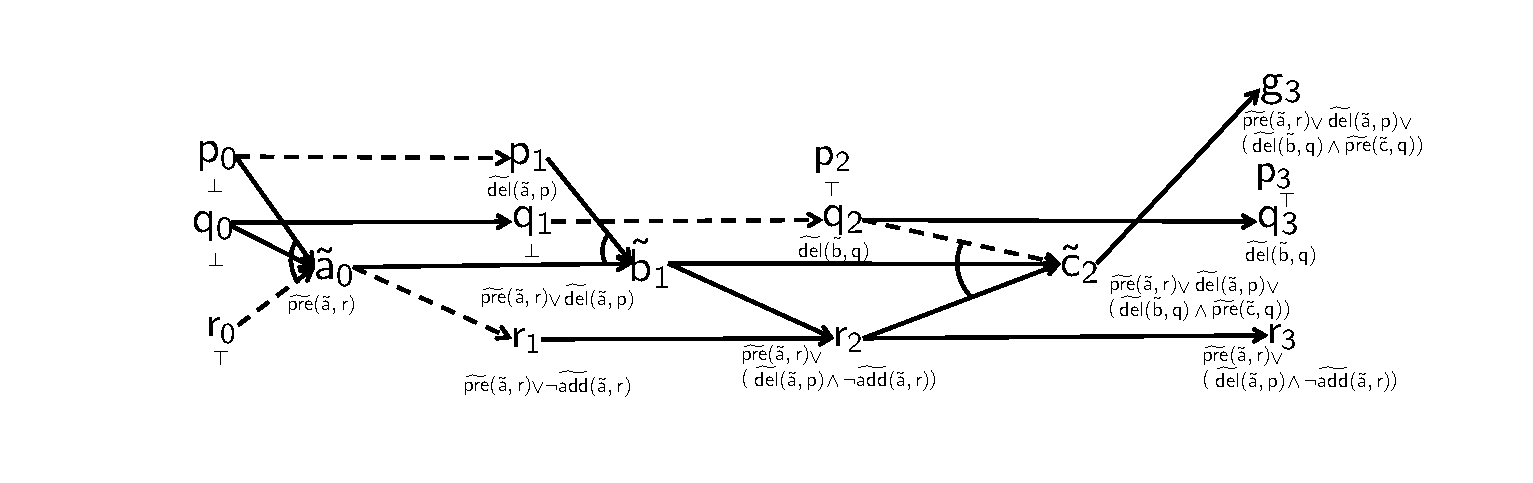
\includegraphics[width=1\linewidth]{WeberBryceICAPS11Fig1.eps}
\vspace*{-1cm}\caption{\label{fig:example} Labeled Plan}
\end{figure*}



\section{Planning in Incomplete Domains}

We present a forward state space planner called \default{} that attempts to
minimize the number of interpretations of the incomplete domain that can result
in plan failure.  \default{} generates states reached under the optimistic
interpretation of the incomplete domain, but labels each state proposition with
the interpretations (a failure explanation) where it will be impossible to
achieve the proposition. As such, the number of interpretations labeling the
goals reached by a plan indicates the number of failed interpretations.  By
counting interpretations (i.e., propositional model counting), we can determine
the quality of a plan.

\default{} labels propositions and actions with domain interpretations that will
respectively fail to achieve the proposition or fail to achieve the
preconditions of an action.  That is, labels indicate the cases where a
proposition will be false (i.e., the plan fails to establish the proposition). 
Labels $d(\cdot)$ are represented as  propositional sentences over ${\sf F}$
whose models correspond to domain interpretations.

Initially, each proposition $p_0 \in s_0$ is labeled $d(p_0) = \perp$ to denote
that there are no failed interpretations affecting the initial state, and each
$p_0 \not\in s_0$ is labeled $d(p_0)=\top$.  For all $t \geq 0$, we define:
\begin{align}
\label{eqn:actlabel}d(\tilde{a}_t) &=  
d(\tilde{a}_{t-1}) \vee \hspace*{-.35cm}\bigvee\limits_{p \in \text{pre}(\tilde{a})}\hspace*{-.39cm} d(p_t) \vee\hspace*{-.35cm} \bigvee\limits_{p \in \widetilde{\text{pre}}(\tilde{a})} \hspace*{-.35cm}(d(p_t)\hspace*{-.09cm}\wedge\hspace*{-.09cm} \widetilde{\text{pre}}(\tilde{a}_t, p)  ) \\
\label{eqn:proplabel}\hspace*{-.1cm}d(p_{t+1}) &= \left\{
\begin{array}{l@{\;}l@{\;}r}
d(p_t) \wedge d(\tilde{a}_t) & : p \in \text{add}(\tilde{a}_t) \\
d(p_t) \wedge  (d(\tilde{a}_t) \vee \\
\hspace*{1.25cm} \neg\widetilde{\text{add}}(\tilde{a}_t, p)) & : p \in \widetilde{\text{add}}(\tilde{a}_t)\\
\top & : p \in \text{del}(\tilde{a}_t)\\
d(p_t) \vee  \widetilde{\text{del}}(\tilde{a}_t, p) 
 &: p \in \widetilde{\text{del}}(\tilde{a}_t)\\
d(p_t) & : \text{otherwise} 
\end{array}
\right. 
\end{align}
\noindent where $d(\tilde{a}_{-1}) = \perp$. The intuition behind the label
propagation is that in Equation \ref{eqn:actlabel} an action will fail  in the
domain interpretations $d(\tilde{a}_t)$ where a prior action failed, a known
precondition is not satisfied, or a possible precondition (which is a known
precondition for the interpretation) is not satisfied. As defined by Equation
\ref{eqn:proplabel}, the plan will fail to achieve a proposition at time $t+1$
in all interpretations where i) the plan fails to achieve the proposition at
time $t$ and the action fails, ii) the plan fails to achieve the proposition at
time $t$ and the action fails or it does not add the proposition in the
interpretation, iii) the action deletes the proposition, iv) the plan fails to
achieve the proposition at time $t$ or in the interpretation the action deletes
the proposition, or v) the action does not affect the proposition and any prior
failed interpretations still apply.

A consequence of our definition of action failure is that each action fails if
any prior action fails.  This definition follows from the semantics that the
state becomes undefined if we apply an action whose preconditions are not
satisfied.  While we use this notion in plan synthesis, we explore the semantics
that the state does not change (i.e., it is defined) upon failure when we
discuss acting in incomplete domains.  The reason that we define action failures
in this manner is that we can determine all failed interpretations affecting a
plan $d(\pi)$, defined  by  $d(\tilde{a}_{n-1}) \vee \bigvee_{g \in G} d(g_n)$.
It is possible to determine the interpretations that fail to successfully
execute the plan up to and including time $t$ by  $d(\tilde{a}_t)$.

For example, consider the plan depicted in Figure \ref{fig:example}.  The
propositions in each state and each action at each time are labeled by the
propositional sentence below it. The edges in the figure connecting the
propositions and actions denote what must be true to successfully execute an
action or achieve a proposition.  The dashed edges indicate that action
incompleteness affects the ability of an action or proposition to support a
proposition.  For example, $\tilde{a}$ possibly deletes $p$, so the edge
denoting its persistence is dashed.  The propositional sentences  $d(\cdot)$
below each proposition and action denote the domain interpretations where a
action will fail or a proposition will not be achieved.  For example,
$\tilde{b}$ at time one, ${\sf \tilde{b}_1}$, will fail if either
$\widetilde{\text{pre}}(\tilde{a}, r)$ or $\widetilde{\text{ del}}(\tilde{a},
p)$ is true in the interpretation.  Thus, $d(\pi) =
\widetilde{\text{pre}}(\tilde{a}, r) \vee \widetilde{\text{del}}(\tilde{a},
p)\vee (\widetilde{\text{del}}(\tilde{b}, q) \wedge
\widetilde{\text{pre}}(\tilde{c}, q))$ and any domain interpretation satisfying
$d(\pi)$ will fail to execute the plan and achieve the goal.




\section{Heuristics in Incomplete Domains}

Similar to propagating failed interpretation labels in a plan, we can propagate
labels in the relaxed planning problem to compute a search heuristic.  The
heuristic is the number of actions in a relaxed plan, and, while we do not use
the number of failed domain interpretations as the primary heuristic, we use the
failure labels to bias the selection of the relaxed plan actions and break ties
between search nodes with an equivalent number of actions in their relaxed
plans.  We solve the relaxed planning problem using a planning graph and 
start with a brief description of planning graphs.

\und{Planning Graph Heuristics}   A relaxed planning graph  is a layered graph
of sets of vertices $({\cal P}_t, {\cal A}_t, ..., {\cal A}_{t+m}, {\cal
P}_{t+m+1})$.  The planning graph built for a state $s_t$ defines ${\cal P}_t =
\{p_t | p \in s_t\}$, ${\cal A}_{t+k} = \{ a_t | \forall_{ p \in \text{pre}(a)}
p_t \in {\cal P}_{t+k}, a \in A \cup A(P)\}$, and ${\cal P}_{t+k+1} =
\{p_{t+k+1} | a_{t+k} \in {\cal A}_{t+k}, p \in \text{add}(a)\}$, for $k = 0,
..., m$.  The set $A(P)$ includes noop actions for each proposition, such that
$A(P) = \{a(p) | p \in P, \text{pre}(a(p)) =\text{add}(a(p))=p,
\text{del}(a(p))=\emptyset\}$. The $h^{FF}$  heuristic
\citep{hoffmann:nebel:jair-01} solves this relaxed planning problem by choosing
actions from ${\cal A}_{t+m}$ to support the goals in ${\cal P}_{t+m+1}$, and
recursively for each chosen action's preconditions, counting the number of
chosen actions.

 
\und{Incomplete Domain Heuristics} Propagating failed interpretations in the
planning graph resembles propagating failed interpretations over a plan.  The
primary difference is how we define the failed interpretations for a proposition
when the proposition has multiple sources of support; recall that we allow only
serial plans and at each time each state proposition is supported by persistence
and/or a single action -- action choice is handled in the search space. In a
level of the relaxed planning graph, there are potentially many actions
supporting a proposition, and {\em we select the supporter with the fewest
failed interpretations}. The chosen supporting action, denoted
$\hat{a}_{t+k}(p)$, determines the failed interpretations affecting a
proposition $p$ at level $t+k+1$.


A relaxed planning graph with propagated labels is a layered graph of sets of
vertices of the form $(\hat{\cal P}_t, \hat{\cal A}_t, ..., \hat{\cal A}_{t+m},
\hat{\cal P}_{t+m+1})$. The relaxed planning graph built for a state
$\tilde{s}_t$ defines $\hat{\cal P}_0 = \{\hat{p}_t | p \in \tilde{s}_t\}$,
$\hat{\cal A}_{t+k} = \{ \hat{a}_{t+k} | \forall_{p \in \text{pre}(\tilde{a})}
\hat{p}_{t+k} \in \hat{\cal P}_{t+k}, \tilde{a} \in \tilde{A} \cup A(P)\}$, and
$\hat{\cal P}_{t+k+1} = \{\hat{p}_{t+k+1} | \hat{a}_{t+k} \in \hat{\cal
A}_{t+k}, p \in \text{add}(\tilde{a}) \cup \widetilde{\text{add}}(\tilde{a})\}$, for $k = 0,
..., m$.  Much like the successor function used to compute next states, the
relaxed planning graph assumes an optimistic semantics for effects by
adding possible add effects to proposition layers, but, as we will explain
below, it associates failed interpretations with the possible adds.

Each planning graph vertex has a label, denoted $\hat{d}(\cdot)$.  The failed
interpretations $\hat{d}(\hat{p}_t) $ affecting a proposition are defined such
that $\hat{d}(\hat{p}_t) = d(p_t)$, and for $k \geq 0$,
\begin{align}
\widehat{d}(\tilde{a}_{t+k}) &= \hspace*{-.2cm} 
\bigvee\limits_{p \in \text{pre}(\tilde{a}) } \hspace*{-.2cm}   \hat{d}(\hat{p}_{t+k}) \vee \hspace*{-.25cm} 
\bigvee\limits_{p \in \widetilde{\text{pre}}(\tilde{a})} \hspace*{-.25cm}  (\hat{d}(\hat{p}_{t+k})  \wedge  \widetilde{\text{pre}}(\tilde{a}, p) )\label{eqn:hact}\\
 \hspace*{-.6cm} \hat{d}(\hat{p}_{t+k+1}) &= 
\left\{\begin{array}{l@{\;}l@{\;}r}
\widehat{d}(\hat{a}_{t+k}(p)) & : p \in \text{add}(\hat{a}_{t+k}(p))\\
\widehat{d}(\hat{a}_{t+k}(p)) \vee \\
\neg\widetilde{\text{add}}(\hat{a}_{t+k}(p), p) & : p \in \widetilde{\text{add}}(\hat{a}_{t+k}(p))\end{array}\right. \hspace*{-.1cm}\label{eqn:hprop}
\end{align}
\noindent Every action in every level $k$ of the planning graph will fail in any
interpretation where their preconditions are not supported (Equation
\ref{eqn:hact}).  A proposition will fail to be achieved in any interpretation
where the chosen supporting action fails to add the proposition (Equation
\ref{eqn:hprop}).

We note that the rules for propagating labels in the planning graph differ from
the rules for propagating labels in the state space.  In the state space, the
action failure labels include interpretations where any prior action fails.  In
the relaxed planning problem, the action failure labels include only
interpretations affecting the action's preconditions, and not prior actions; it
is not clear which actions will be executed prior to achieving a proposition
because many actions may be used to achieve other propositions at the same time.

\und{Heuristic Computation}   We terminate the relaxed planning graph expansion
at the level $t+k+1$ where one of the following conditions is met: i) the
planning graph reaches a fixed point where the explanations do not change,
$\hat{d}(\hat{p}_{t+k}) = \hat{d}(\hat{p}_{t+k+1})$ for all $p\in P$, or ii) the
goals have been reached at $t+k+1$ and the fixed point has not yet been reached.
Our $h^{\sim FF}$ heuristic makes use of the chosen supporting action
$\hat{a}_{t+k}(p)$ for each proposition that requires support in the relaxed
plan, and, hence, measures the number of actions used while attempting to
minimize failed interpretations (the supporting actions are chosen by comparing
failure explanations). The other heuristic $h^{\sim M}$ measures the number of
interpretations that fail to reach the goals in the last level (i.e., such that
$h^{\sim M} = |M(\vee_{p \in G} \hat{d}(\hat{p}_{t+m+1}))|$, where $m+1$ is the
last level of the planning graph, $M(\cdot)$ is the set of models of a formula.
\default{} uses both heuristics, treating $h^{\sim FF}$ as the primary heuristic
and using $h^{\sim M}$ to break ties. While it is likely that swapping the role
of the heuristics may lead to better quality plans (fewer failed
interpretations), our informal experiments determined that the scalability of
\default{} is greatly limited in such cases; measuring failed interpretations is
not correlated with solution depth in the search graph unlike relaxed plan
length.  The relaxed plans are informed by the propagated explanations because
we use the failure explanation to bias action selection.

\section{Counting Models \& Prime Implicants }

Failure explanations $d(\cdot)$ and $\hat{d}(\cdot)$ are propositional sentences
that help bias decisions in search and heuristics.  Namely, we assume that we
can count the number of propositional models of these sentences to indicate how
many interpretations of the incomplete domain will fail to successfully execute
a plan.  Model counting is intractable \citep{Roth96}, but by representing the
sentences as OBDDs \citep{bryant-ieeetc86}, model counting is polynomial in the
size of the OBDD \citep{darwiche} (which can be exponential sized in the worst
case).

In addition to OBDDs and model counting, we also explore counting prime
implicants (PIs) -- also called diagnoses -- which allows us to computer a
heuristic $h^{\sim PI}$, which is similar to $h^{\sim M}$. A set of PIs is a set
of conjunctive clauses (similar to a DNF) where no clause is subsumed by another, and are used in model-based diagnosis to represent diagnoses (sets of incomplete features
that must interact to cause system failure) \citep{dekleer}.  We find it useful
to bound the cardinality (the number of conjuncts) of the PIs, effectively
over-approximating the models of a propositional sentence.

Instead of counting the models of two labels $d(\cdot)$ and $d'(\cdot)$, we can
compare the number of PIs (as in $h^{\sim PI}$).  Our intuition is that having
fewer diagnoses of failure is preferred, just as is having fewer models of failure (even though
having fewer PIs does not always imply fewer models).  The advantage is that
counting PIs is much less expensive than counting models, especially if we bound
the cardinality of the PIs.  Finally, we use a heuristic when counting PIs
whereby we compare two sets in terms of the number of cardinality-one PIs, and
if equal, the number of cardinality-two PIs, and so on.  The intuition behind
comparing PIs in this fashion is that smaller PIs are typically satisfied by a
larger number of models and are thus more representative.  That is, a sentence
with one cardinality-one PI will have more models than a sentence with one
cardinality-two PI.

\section{Acting in Incomplete Domains} Acting in incomplete domains provides an
opportunity to learn about the domain by observing the states resulting from
execution.  In the following, we describe what our agent \goalie{} can
learn from acting in incomplete domains and how it  achieves its goals.
\goalie{} will continue to execute a plan until it is faced with an action that
is guaranteed to fail or it has determined that the plan failed in hindsight.

\goalie{} maintains a propositional sentence $\phi$ defined over ${\sf
F} \cup \{fail\}$ which describes the current knowledge of the
incomplete domain.  The proposition $fail$ denotes whether \goalie{} believes
that its current plan failed -- it is not always possible to determine if an
action applied in the past did not have its preconditions satisfied.  Initially,
\goalie{} believes $\phi = \top$, denoting its complete lack of knowledge of the
incomplete domain and whether its current plan will fail.    If \goalie{}
executes  $\tilde{a}$ in state $s$ and transitions to state $s'$, then it 
updates its knowledge as $\phi \wedge o(s, \tilde{a}, s')$, where
\noindent \begin{eqnarray}
o(s, \tilde{a}, s') &=& \left\{ \begin{array}{ll}
(fail \wedge o^-) \vee  o^+  &: s = s'\\
o^+  & : s \not= s'
\end{array}\right. \label{eqn:update}\\
o^- &=& \bigvee\limits_{\substack{\widetilde{\text{pre}}(\tilde{a},p) \in {\sf F}:\\ p \not\in s} } \widetilde{\text{pre}}(\tilde{a},p) \label{eqn:update1} \\
o^+ &=& o^{pre} \wedge o^{add} \wedge o^{del}\label{eqn:update2}\\
o^{pre} &=& \bigwedge\limits_{\substack{\widetilde{\text{pre}}(\tilde{a},p) \in
{\sf F}:\\ p \not\in s} }\hspace*{-0.25cm}\neg \widetilde{\text{pre}}(\tilde{a},p)\label{eqn:update3}  \\ o^{add} &=&  \hspace*{-.5cm}\bigwedge\limits_{\substack{\widetilde{\text{add}}(\tilde{a},p) \in {\sf F}:\\ p\in s'\backslash s} }\hspace*{-0.25cm}\widetilde{\text{add}}(\tilde{a},p)   \wedge  \hspace*{-0.5cm}\bigwedge\limits_{\substack{\widetilde{\text{add}}(\tilde{a},p) \in {\sf F}: \\ p \not\in  s\cup s'}} \hspace*{-0.25cm}\neg \widetilde{\text{add}}(\tilde{a},p)   \label{eqn:update4}\\
o^{del} &=& \hspace*{-.5cm} \bigwedge\limits_{\substack{\widetilde{\text{del}}(\tilde{a},p) \in {\sf F}: \\p \in s \backslash s'}} \hspace*{-0.25cm}\widetilde{\text{del}}(\tilde{a},p)  \wedge  \hspace*{-0.5cm}\bigwedge\limits_{\substack{\widetilde{\text{del}}(\tilde{a},p) \in {\sf F}:\\ p \in s\cap s'}} \hspace*{-0.25cm}\neg \widetilde{\text{del}}(\tilde{a},p)  \label{eqn:update5}
\end{eqnarray}
\noindent We assume that the state will remain unchanged when \goalie{} executes
an action whose precondition is not satisfied by the state, and because the
state is observable, Equation \ref{eqn:update} references the case where the
state does not change and the case where it changes.  If the state does not
change, then either the action failed and one of its unsatisfied possible
preconditions is a precondition (Equation \ref{eqn:update1}) or the action
succeeded (Equation \ref{eqn:update2}).  If the state changes, then \goalie{}
knows that the action succeeded.  If an action succeeds, \goalie{} can conclude
that i) each possible precondition that was not satisfied is not a precondition
(Equation \ref{eqn:update3}), ii) each possible add effect that appears in the
successor but not the predecessor state is an add effect and each that does not
appear in either state is not an add effect, iii) each possible delete effect
that appears in the predecessor but not the successor is a delete effect and
each that  appears in both states is not a delete effect.

Using $\phi$, it is possible to determine if the next action in a plan, or any
subsequent action, can or will fail.  If  $\phi \wedge d(\tilde{a}_{t+k})$ is
satisfiable, then $\tilde{a}_{t+k}$ {\em can} fail, and if $\phi \models
d(\tilde{a}_{t+k})$, then $\tilde{a}_{t+k}$ {\em will}  fail.  \goalie{} will
execute an action if it may not fail, even if later actions in its plan will
fail.  If \goalie{} determines that its next action will fail, or a prior action
failed ($\phi \models fail$), then it will re-plan.  \goalie{}  uses $\phi$ to
modify the actions during re-planning by checking for each incomplete domain
feature $f \in {\sf F}$ if $\phi \models f$ or if $\phi \models \neg f$.  Each
such literal entailed by $\phi$ indicates if the respective action has the
possible feature as a known or impossible feature; all other features remain as
possible features.



\begin{algorithm}[t]
\SetLine
\KwIn{state $s$, goal $G$, actions $\tilde{A}$}
 $\phi \leftarrow \top$; $\pi \leftarrow Plan(s, G, \tilde{A}, \phi)$\;
\While{$\pi \not= ()$ and $G\not\subseteq s$}{
 $\tilde{a} \leftarrow \pi.first()$;
 $\pi \leftarrow \pi.rest()$\;
\eIf{$\text{pre}(\tilde{a}) \subseteq s$ and $\phi \not\models \bigvee\limits_{\substack{\widetilde{\text{pre}}(\tilde{a},p) \in {\sf F}: p \not\in s} } \widetilde{\text{pre}}(\tilde{a},p)
$}{
	$s ' \leftarrow Execute(\tilde{a})$\;
	 $\phi \leftarrow \phi \wedge o(s, \tilde{a}, s')$\;
	 $s \leftarrow s'$\;
}
{
	 $\phi \leftarrow \phi \wedge fail$\;
}

\If{$\phi \models fail$ }{
	 $\phi \leftarrow \exists_{fail}  \phi$\;
	 $\pi \leftarrow Plan(s, G, \tilde{A}, \phi)$\;
}
}
\caption{\goalie{}$(s, G, \tilde{A})$}\label{alg:replan}
\end{algorithm}

Algorithm \ref{alg:replan} is the strategy used by \goalie{}.  The algorithm
involves initializing the agent's knowledge and plan (line 1), and then while
the plan is non-empty and the goal is not achieved (line 2) the agent proceeds
as follows.  The agent selects the next action in the plan (line 3) and
determines if it can apply the action (line 4).  If it applies the action, then
the next state is returned by the environment/simulator (line 5) and the agent
updates its knowledge (line 6 and Equation \ref{eqn:update}) and state (line 7),
otherwise the agent determines that the plan will fail (line 9).  If the plan
has failed (line 11), then the agent forgets its knowledge of the plan failure
(line 12) and finds a new plan using its new knowledge (line 13). \goalie{} is
not guaranteed success, unless it can find a plan that will not fail (i.e., 
$d(\pi) = \perp$).

\goalie{} is not hesitant to apply actions that may fail because trying actions
is its only way to learn about them.  However, \goalie{} is able to determine
when actions will fail and re-plans.  More conservative strategies are possible
if we assume that \goalie{} can query a domain expert about action features
to avoid potential plan failure, but we leave such goal-directed knowledge
acquisition for future work.


\section{Empirical Evaluation}\label{sec:empirical}

The empirical evaluation is divided into four sections:  the domains used for
the experiments, the test setup used, results for off-line planning, and results
for on-line planning and execution.  The questions that we would like to answer
include:
\begin{packed_itemize}
\item Q1: Does reasoning about incompleteness lead to high quality plans?
\item Q2: Does counting prime implicants perform better than counting models?
\item Q3: As the number of incomplete features grows, does stronger reasoning
about incompleteness help?
\item Q4: Does reasoning about incompleteness reduce the number of
execution failures during execution?
\end{packed_itemize}





\und{Domains} We use four domains in the evaluation: a modified Pathways,
Bridges,  a modified PARC Printer, and Barter World.  In
all domains, we derived multiple instances by randomly (with probabilities 0.25,
0.5, 0.75, and 1.0 for each action) injecting incomplete  features.   
With these variations of the domains, the instances include up to ten thousand
incomplete  features each. All planning results are taken from ten random
instances (varying $\sf F$) of each problem and within these, each planning
and execution result is one of ten ground-truth domains selected by the
simulator. The problem generators and our planner are available at:
http://www.cs.usu.edu/$\sim$danbryce/software/default.jar.

The Pathways (PW) domain from the International Planning Competition  (IPC)
involves actions that model chemical reactions in signal transduction pathways. 
Pathways is a naturally incomplete domain where the lack of knowledge of the
reactions is quite common because they are an active research topic in biology.

The Bridges (BR) domain, of which there are three versions, consists of a
traversable grid and the task is to find a different treasure at each corner of
the grid. In BR1 (version 1), a bridge might be required  to cross between some
grid locations (a possible precondition); additionally in BR2, many of the
bridges may have a troll living underneath that will take all the treasure
accumulated (a possible delete effect); and additionally in BR3, the corners may
give additional treasures (possible add effects).  Grids are square and vary in
dimension (2-16).

The PARC Printer (PP) domain from the IPC involves planning paths for sheets of
paper through a modular printer.  A source of domain incompleteness is that a
module accepts only certain paper sizes, but its documentation is incomplete. 
Thus, paper size becomes a possible precondition to actions using the module.

The Barter World (BW) domain involves navigating a grid and bartering items to
travel between locations.  The domain is incomplete because actions that acquire
 items are not always known to be successful (possible add effects) and
 traveling between locations may require
certain items (possible preconditions) and may result in the loss of an item
(possible delete effects). Grids vary in dimension (2-16) and items in number
(1-4).




   

\und{Test Setup} The tests were run on a Linux machine with a 3 Ghz Xeon
processor, a memory limit of 2GB, and a time limit of 20 minutes per run for the
off-line planning invocation and 60 minutes for each on-line planning and
execution invocation.  All code was written in Java and run on the 1.6 JVM. 
\default{} uses a greedy best first search with deferred heuristic evaluation
and a dual-queue for preferred and non-preferred operators
\citep{DBLP:journals/jair/Helmert06}.  


   
We use five configurations of the planner: \default{}-$FF$, \default{}-$PIk$ (k
= 1, 2, 3), and \default{}-$BDD$, that differ in how they reason about domain
incompleteness.  \default{}-$FF$ does not compute failure explanations and uses
the FF heuristic;  it is inspired by the planner used by CA because it is likely
to find a plan that will work for only the most optimistic domain
interpretation.  \default{}-$PIk$, where $k$ is the bound on the cardinality of
the prime implicants, counts prime implicants to compare failure
explanations.  \default{}-$BDD$ uses OBDDs to represent and count failure
explanations.  The number of failed interpretations for a plan $\pi$ found by
any of the planners is found by counting models of an OBDD
representing $d(\pi)$. The versions of the planner are compared by the
proportion of interpretations of the incomplete domain that achieve the goal and
total planning time in seconds. The plot in the following section depict these
results using the cumulative
planning time to identify the performance over all problems and domains.  We
also report detailed results on the number of solved problems per domain and the
relative quality of solutions (successful domain interpretations).


\begin{table}[t]
\centering 
\begin{tabular}{|l|rrrrr|}      \hline &  FF  & PI1 & PI2  &  PI3  &  BDD  \\\hline
FF	&		0		&		155		&		161		&		161		&		123		\\
PI1	&	{\bf	629}	&		0		&	{\bf	79}	&	{\bf	78}	&	{\bf	208}	\\
PI2	&	{\bf	619}	&		77		&		0		&		46		&	{\bf	208}	\\
PI3	&	{\bf	594}	&		62		&	{\bf	51}	&		0		&	{\bf	199}	\\
BDD & {\bf 512} &  189  &  189  &  187  &  0  \\\hline
\end{tabular}																						
\caption{\label{tab:qualcomp} Number of plans having a greater
number of successful domain interpretations (i.e., better quality).} 
\end{table}

\begin{figure}[t]\centering
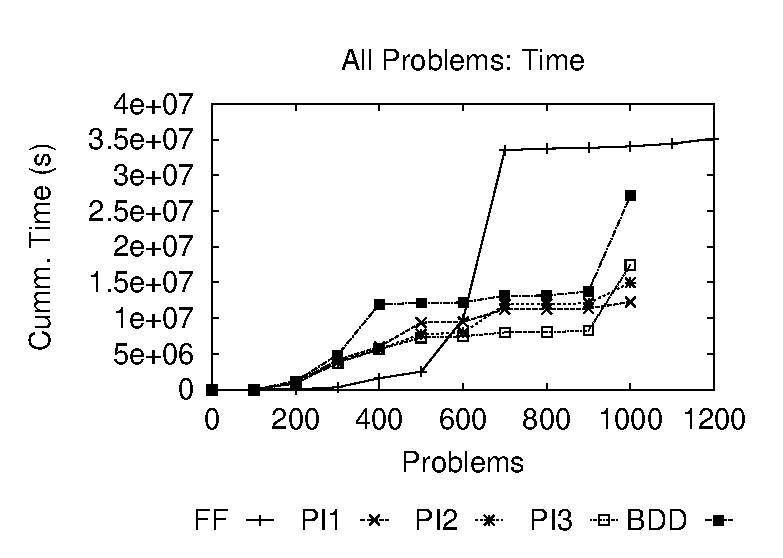
\includegraphics[width=\linewidth]{WeberBryceICAPS11Fig2.eps}
\caption{\label{fig:alltotaltime}Cumulative Time  in  All Domains.}
\end{figure} 

We also compare the off-line planning results to a conformant probabilistic
planner POND (with N=10 particles in its heuristic) \citep{aij-mclug} that solves
translated instances of the incomplete STRIPS problems.  We set the minimum
required probability of goal satisfaction to the minimum proportion of
successful domain interpretations of plans found by the other approaches. We do
not provide the details of the translation because the results are very poor,
but refer the reader to an extended version of this work
\citep{USU-CS-TR-11-001}.  We attempted a comparison to PFF \citep{pff}, but the
implementation proved unstable for all but the smallest instances.


\begin{table}[t]				\centering																				
\begin{tabular}{|l|r|r@{ }r@{ }r@{ }r|r|}																								
\hline																								
Domain	&		FF		&		PI1		&		PI2		&		PI3		&		BDD		&	POND	\\ \hline	\hline
PP 0.25	&		130		&		83		&		85		&	{\bf	86}	&		80		&	10	\\	
PP 0.5	&		130		&		87		&	{\bf	88}	&		87		&		80		&	0	\\	
PP 0.75	&		130		&		82		&	{\bf	83}	&		81		&		80		&	0	\\	
PP 1.0	&		13		&	{\bf	10}	&		9		&		9		&		8		&	0	\\	\hline
PP	&		403		&		262		&	{\bf	265}	&		263		&		248		&	10	\\	\hline\hline
BR1 0.25 	&		40		&	{\bf	22}	&	{\bf	22}	&	{\bf	22}	&	{\bf	22}	&	2	\\	
BR1 0.5 	&		39		&	{\bf	20}	&	{\bf	20}	&	{\bf	20}	&	{\bf	20}	&	2	\\	
BR1 0.75 	&		36		&	{\bf	19}	&	{\bf	19}	&	{\bf	19}	&	{\bf	19}	&	2	\\	
BR1 1.0 	&		4		&	{\bf	2}	&	{\bf	2}	&	{\bf	2}	&	{\bf	2}	&	1	\\	
BR2 0.25 	&		38		&		20		&		20		&		20		&	{\bf	21}	&	3	\\	
BR2 0.5 	&		35		&	{\bf	25}	&	{\bf	25}	&	{\bf	25}	&		23		&	3	\\	
BR2 0.75 	&		35		&	{\bf	22}	&		21		&		21		&		21		&	2	\\	
BR2 1.0 	&		4		&	{\bf	2}	&	{\bf	2}	&	{\bf	2}	&	{\bf	2}	&	1	\\	
BR3 0.25 	&		45		&	{\bf	36}	&	{\bf	36}	&	{\bf	36}	&	{\bf	36}	&	1	\\	
BR3 0.5 	&		47		&	{\bf	33}	&	{\bf	33}	&	{\bf	33}	&		32		&	2	\\	
BR3 0.75 	&		46		&		39		&		39		&		39		&	{\bf	41}	&	1	\\	
BR3 1.0 	&		5		&	{\bf	4}	&	{\bf	4}	&	{\bf	4}	&		3		&	1	\\	\hline
BR 	&		374		&	{\bf	244}	&		243		&		243		&		242		&	21	\\	\hline\hline
BW 0.25 	&		150		&		106		&		128		&	{\bf	129}	&		108		&	60	\\	
BW 0.5 	&		150		&		134		&	{\bf	137}	&		134		&		118		&	45	\\	
BW 0.75 	&		150		&	{\bf	140}	&		138		&		137		&		111		&	27	\\	
BW 1.0 	&		15		&	{\bf	14}	&	{\bf	14}	&	{\bf	14}	&		11		&	2	\\	\hline
BW 	&		465		&		394		&	{\bf	417}	&		414		&		348		&	155	\\	\hline\hline
PW 0.25 	&		160		&	{\bf	40}	&	{\bf	40}	&	{\bf	40}	&	{\bf	40}	&	19	\\	
PW 0.5 	&		160		&	{\bf	70}	&		60		&		50		&		60		&	13	\\	
PW 0.75 	&		170		&	{\bf	60}	&		50		&		40		&	{\bf	60}	&	12	\\	
PW 1.0 	&		19		&		5		&		6		&		6		&	{\bf	7}	&	2	\\	\hline
PW 	&		509		&	{\bf	175}	&		156		&		136		&		167		&	46	\\	\hline\hline
Total	&		1751		&		1075		&	{\bf	1081}	&		1056		&		1005		&	232	\\	
\hline																								
\end{tabular}	\caption{\label{tab:solved} Instances Solved By Domain}																							
\end{table}																																												



\und{Off-line Planning Results} Figure \ref{fig:alltotaltime} plots the
 cumulative total planning time.  To enhance readability, every one
hundredth data point is plotted in the figures (while still representative of
the true cumulative number).  Table \ref{tab:qualcomp} lists the number of times
that the configuration in the row finds a better solution (number of successful
interpretations) than the configuration in the column when both solve a problem,
with the best of each pair bolded. Table \ref{tab:solved} lists the number of solved problems for each planner and
highlights the most solved for each domain in bold.

We see that Q1 is answered positively by the results.  Plan quality is
improved by reasoning about incompleteness (through \default{}-$PIk$ or -$BDD$),
but scalability suffers.  However, we note that minimizing the number of failed
interpretations  can be phrased as a conformant probabilistic
planning problem, which is notoriously difficult \citep{pff,aij-mclug}, and
expecting the scalability of a classical planner is perhaps  unreasonable.

Q2 is answered overall positively by our experiments because the $PIk$ counting
approaches solve more problems with better quality and in less time than the
$BDD$ model counting approach.  

Q3 is answered negatively because as the probability of injecting incomplete
features grows from 0.25 to 1.0 the $PI3$ approach initially solves the most
problems, but then $PI2$, and then $PI1$ solve the most problems in each domain.
A possible explanation for this result is that it becomes too costly to reason
about incompleteness as it increases and that a more coarse approach is needed;
however, the $BDD$ approach while not the best, seems to degrade less as the
incompleteness increases.  It is likely that the OBDD package 
implementation \citep{jdd} is to credit for the $BDD$ approach's performance
because model counting can become prohibitively expensive in larger problems.

Table \ref{tab:solved} indicates that POND is not competitive and suggests that
existing approaches are not directly applicable to planning in incomplete
domains.  We note that \default{} is inspired by POND, but employs more
approximate reasoning about incompleteness by using bounded prime implicants
(see \citep{USU-CS-TR-11-001} for a more thorough discussion). 

 
  
\begin{figure*}[t]    
\hspace*{-1cm}
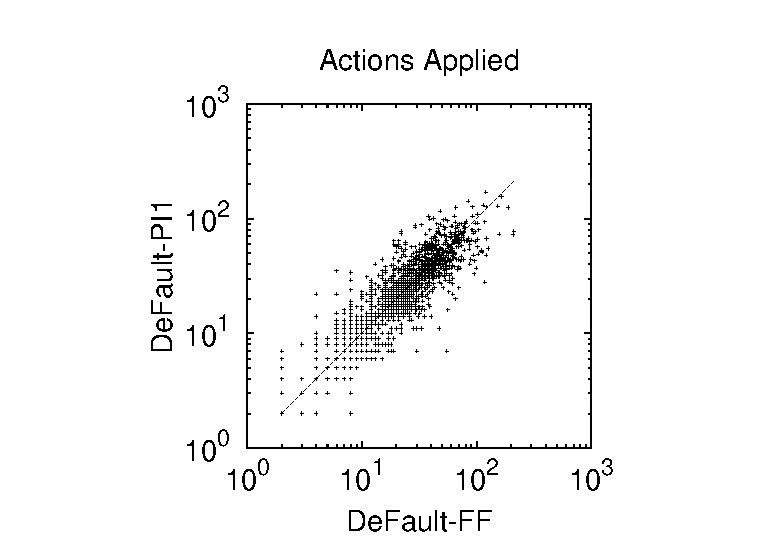
\includegraphics[width=.42\linewidth]{./WeberBryceICAPS11Fig3a.eps}\hspace*{-1.5cm}
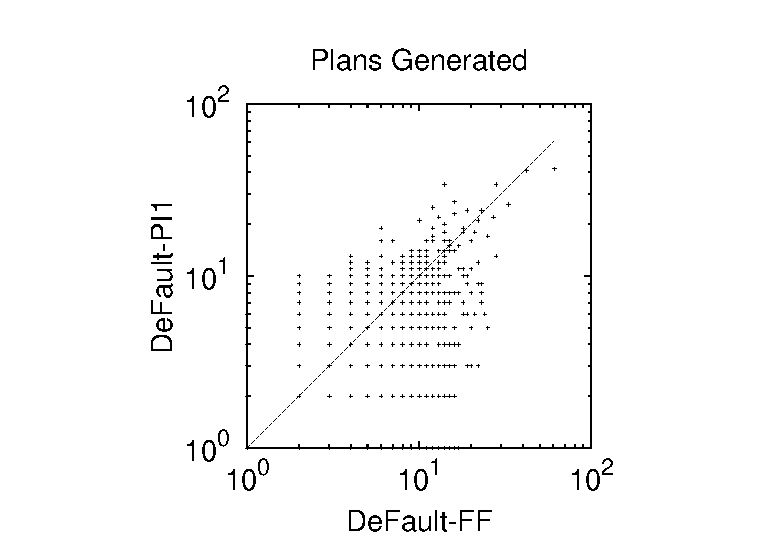
\includegraphics[width=.42\linewidth]{./WeberBryceICAPS11Fig3b.eps}\hspace*{-1.5cm}
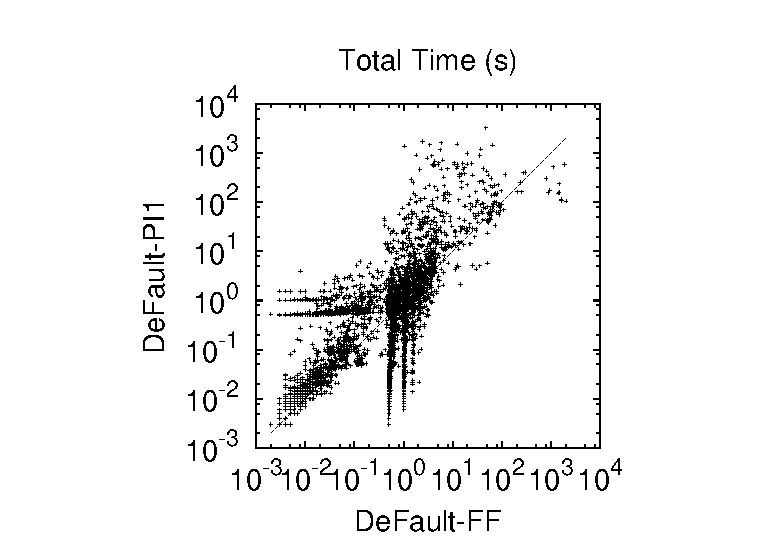
\includegraphics[width=.42\linewidth]{./WeberBryceICAPS11Fig3c.eps} 
\caption{\label{fig:exec} Comparison of Goalie with \default-$FF$ and
\default-$PI1$.}
\end{figure*}		   

 

\und{On-line Planning \& Execution Results} Figure \ref{fig:exec} depicts a
comparison between Goalie using \default{}-$FF$ and \default{}-$BDD$ to
synthesize plans, so that we can judge whether planning and execution strategies
such as that of CA will benefit when planners reason about incompleteness.  The
scatter plots in the figure show the respective number of actions applied to
achieve the goal, the number of plans generated, and the total planning and
execution time.

Q4 is answered mostly positively. By investigating the plots of the number of
actions taken and the number of plans generated, it is apparent that
\default-$PI1$ takes fewer actions as the instances require near 100 steps, and
tends to re-plan less often. The plot of the total time taken shows that the
planners are somewhat mixed or even for times less than 10 seconds.  However,
for times greater than 10 seconds, it appears that using \default-$FF$ in
\goalie{} can take up to an order of magnitude less time.  However, there are
several difficult instances in which \default-$PI1$ does outperform
\default-$FF$.    We expect that more efficient implementations of reasoning
about prime implicants (e.g., tries) could lower the cost of planning with
\default{}, making it able to capitalize on its better quality plans.
 

\section{Related Work}

Planning in incomplete domains is noticeably similar to planning with incomplete
information, where action descriptions instead of states are incomplete. 
Incomplete domains can be translated to conformant probabilistic planning
domains, and planners such as POND \citep{aij-mclug} and PFF \citep{pff} are
applicable.  However, while the translation is theoretically feasible, current
CPP planners are not reasonable approaches to the problem.  
 

Our investigation is an instantiation of model-lite planning \citep{modellite}.
Constraint-based hierarchical task networks are an alternative, pointed out by
\citet{modellite},  which avoid specifying all preconditions and effects through
methods and constraints that correspond to underlying, implicit causal links.

As previously stated, this work is a natural extension of the \citet{Garland02}
model for evaluating plans in incomplete domains.  Our methods for computing
plan failure explanations are slightly different in that we compute them in the
forward direction and allow for multiple, interacting faults instead of the
single faults.  In addition to calculating the failure explanations of partial
plans, we use a relaxed planning heuristic informed by failure
explanations.

Prior work of \citet{DBLP:conf/aips/ChangA06} addresses planning with incomplete
models, but does not attempt to synthesize robust plans, which is similar to our
\default{}-$FF$ planner.  We have shown that incorporating knowledge about
domain incompleteness into the planner can lead to an agent that re-plans less. 
We also differ in that we do not assume direct feedback from the environment about
action failures and we can learn action preconditions.

\section{Conclusion}

We have presented the first work to address planning in incomplete domains as
heuristic search to find robust plans.  Our planner, \default{}, i) performs
forward search while maintaining plan failure explanations, and ii) estimates
the future failures by propagating failure explanations on planning graphs.  We
have shown that, compared to a configuration that essentially ignores aspects of
the incomplete domain, \default{} is able to scale reasonably well but find much
better quality plans.  We have also shown that representing plan failure
explanations with prime implicants leads to better scalability than counting
OBDDs models.  Our agent \goalie{} uses \default{} to generate robust plans that
fail less often and require less re-planning than more optimistic planning
approaches that ignore  incompleteness.


\und{Acknowledgements} This work was supported by DARPA contract HR001-07-C-0060.

\bibliography{WeberBryceICAPS11}
\bibliographystyle{aaai}
 
\end{document}
